\setcounter{rownumber}{0}
\chapter{Laser Cooling of Traveling-Wave Phonons in an Optical Fiber}
\label{ch:Cooling}
\acresetall

Joel N. Johnson\footnote{\label{Cooling-NAU}
Department of Applied Physics and Materials Science, Northern Arizona University, Flagstaff, AZ 86011, USA}%
\textsuperscript{,}\footnote{\label{Cooling-MIRA}
Center for Materials Interfaces in Research and Applications, Flagstaff, AZ 86011, USA},
Danielle R. Haverkamp\textsuperscript{\ref{Cooling-NAU},\ref{Cooling-MIRA}},
Yi-Hsin Ou\footnote{\label{Cooling-UofA}
College of Optical Sciences, University of Arizona, Tucson, AZ, USA},
Khanh Kieu\textsuperscript{\ref{Cooling-UofA}},
Nils T. Otterstrom\footnote{\label{Cooling-Sandia}
Photonic and Phononic Microsystems, Sandia National Laboratories, Albuquerque, New Mexico, USA},
Peter T. Rakich\footnote{\label{Cooling-Yale}
Department of Applied Physics, Yale University, New Haven, CT, USA},
Ryan O. Behunin\textsuperscript{\ref{Cooling-NAU},\ref{Cooling-MIRA}}

\hfill

\textit{This chapter elaborates on experiments and results related to the demonstration of optomechanical cooling of traveling wave phonons in an optical fiber, which have been published as an article by the same name in Physical Review Applied by Johnson et al. (2023) \cite{johnson2023laser}. Any discrepancies, omissions, or errors that may exist between the published paper and this dissertation chapter are the sole responsibility of the author, as the text, analyses, and interpretations herein represent an independent and original presentation of the work.}

%--------------------------------------------------------------------%

\section{Introduction}
\label{Cooling:sec:Introduction}

Laser cooling has profoundly transformed modern \ac{AMO} physics, enabling unprecedented control over the motion of ions, atoms, and molecules. From the earliest proposals and demonstrations of Doppler cooling in dilute gases \cite{hansch1975cooling} to the realization of ultracold quantum gases in Bose–Einstein condensates\cite{anderson1995observation}, the ability to reduce thermal motion with light underpins breakthroughs ranging from high-precision atomic clocks to quantum state preparation\cite{ludlow2015optical}. Equally impactful is the extension of laser cooling concepts into solid-state systems. In rare-earth-doped optical crystals, for example, anti-Stokes fluorescence cooling has now approached cryogenic temperatures, cooling Yb-doped solids down to \(\sim\)\SI{87}{\kelvin} (the boiling point of liquid argon) and projected to reach \SI{77}{\kelvin} (liquid nitrogen) in the near future. \cite{meng2018realization} Such optical refrigeration offers a vibration-free route to cryocoolers and has steadily advanced since the first demonstration in 1995. \cite{epstein1995observation} Meanwhile, in mesoscopic mechanics, radiation-pressure laser cooling of solid-state oscillators has opened new frontiers. By coupling light to discrete mechanical modes in optical or microwave cavities, researchers can damp mechanical vibrations to the point of quantum ground-state occupancy. \cite{chan2011laser} Milestone experiments achieved sub-single-phonon populations in nanomechanical resonators cooled by laser light\cite{chan2011laser}, laying the groundwork for quantum metrology and hybrid quantum devices. From \ac{AMO} systems to solid-state platforms, laser cooling has become a cornerstone technique for reducing thermal noise and accessing novel quantum regimes.

Given this context, there is intense interest in applying laser cooling to optomechanical systems, where light interacts with vibrational modes of a material. The established paradigm in optomechanics involves discrete mechanical oscillators coupled to optical cavities. \cite{aspelmeyer2014cavity} In a typical cavity-optomechanical system, e.g., a tiny mirror or membrane attached to a cavity, the radiation pressure force provides a parametric coupling between an optical resonance and a mechanical mode. \cite{aspelmeyer2014cavity} By tuning a laser slightly red of a cavity resonance (i.e. the anti-Stokes sideband), photons can scatter inelastically from the mechanical vibration, gain energy (up-shift) by absorbing a phonon, and promptly leave the cavity, carrying away thermal energy. This sideband cooling process leads to a reduced phonon population in the mechanical mode, provided the anti-Stokes scattering dominates over the Stokes (down-shift) process that would add phonons. Using this approach, a variety of mechanical oscillators from gram-scale mirrors to nanoscale beams have been cooled near their ground state of motion. \cite{chan2011laser} A landmark example is the laser cooling of a \SI{3.7}{\giga\hertz} silicon nanobeam mode to an average occupancy of \(\langle n\rangle \approx 0.85\) (15\% of one quantum) starting from \SI{20}{\kelvin} environment. \cite{chan2011laser} Such achievements, along with comprehensive theoretical frameworks\cite{aspelmeyer2014cavity}, firmly established the state-of-the-art: \emph{discrete} mechanical modes can be laser-cooled via engineered light–matter interactions in optical cavities.

Early optomechanical cooling experiments focused on isolated resonant modes, but recent work has pushed toward cooling \emph{continuum} vibrational degrees of freedom, in particular, traveling-wave phonons in extended media. One route to bridging this gap is to use \ac{WGM} microresonators, which support both localized optical modes and traveling acoustic waves confined around the periphery. In 2012, Bahl et al. demonstrated the first observation of Brillouin optomechanical cooling in a silica microcavity. \cite{bahl2012observation} In that system, light circulating in the \ac{WGM} resonator underwent spontaneous Brillouin scattering with an acoustic whispering-gallery wave. Because the scattering was in the forward direction (co-propagating light and sound), it accessed a low-frequency acoustic mode that had much lower damping than the usual high-frequency phonons of spontaneous backscattering. Satisfying this low acoustic dissipation condition (achieving phonon lifetimes longer than the optical storage time) allowed the optical field to cool the mechanical mode rather than amplify it. The experiment revealed two regimes: the normal Stokes process where light amplifies acoustic vibrations, and a Brillouin cooling regime where anti-Stokes scattering dominantly \emph{damps} the acoustic motion. This result was remarkable since Brillouin interactions in bulk or fiber had long been known primarily as a heating (Stokes) process; the microresonator provided the multi-mode, low-loss environment needed to tip the balance towards net cooling.

Even more surprising was the recent demonstration that one can cool a continuum of phonon modes in a completely non-resonant, traveling-wave configuration. \cite{otterstrom2018optomechanical} Otterstrom et al. (2018) showed for the first time that laser cooling is possible in a continuous optomechanical waveguide, without any optical cavity or discrete mechanical resonance. In their experiment, light propagating through a \SI{2.3}{\centi\meter} silicon photonic waveguide was observed to reduce the thermal occupancy of a band of acoustic phonons via Brillouin scattering. The key was to leverage intermodal Brillouin scattering, wherein the pump laser in one waveguide mode scatters to an anti-Stokes photon in a different optical mode while annihilating a phonon. This phase-matched anti-Stokes process selectively damped those phonons, cooling a spectral band by over \SI{30}{\kelvin} relative to room temperature. Conceptually, the continuous-waveguide regime has an inherent advantage: the Stokes (phonon-creating) and anti-Stokes (phonon-annihilating) processes occur on different phonon modes in an extended medium. Thus, any unavoidable Stokes scattering does not re-excite the very phonon mode being cooled, avoiding the direct competition that limits cooling of a single isolated mode. Still, achieving net cooling in a traveling-wave system demands stringent conditions. The optical wave must interact sufficiently strongly with the acoustic waves (high acousto-optic coupling), and the phonons must remain dissipated long enough for the cooling scattering to outpace thermal re-population and for the light to exit the system carrying that stolen mechanical energy with it. In the silicon waveguide used by Otterstrom et al., engineered cross-section geometry provided large Brillouin gain, and the small device length ensured that anti-Stokes photons escaped the system faster than the phonons could dissipate, fulfilling these requirements. \cite{otterstrom2018optomechanical} This demonstration has spurred growing interest in continuous optomechanical cooling, including new theoretical proposals to dynamically control phonon baths in waveguide systems. \cite{zhu2023dynamic}

\textit{Laser cooling of traveling-wave phonons in an optical fiber} is a natural next goal in this progression. Optical fibers represent the quintessential one-dimensional continuous medium for light and sound, with applications ranging from fiber lasers to quantum information transfer. Cooling phonons in fiber could, for example, suppress thermally driven noise (e.g. guided-acoustic-wave Brillouin noise) that limits the frequency stability of fiber lasers and squeezes light in fiber interferometers. \cite{shin2015control} It could also enable new in-fiber acousto-optic devices with reduced thermal noise, or even allow one to prepare traveling phonon wavepackets in low-entropy states for quantum phononics. However, extending optomechanical cooling to standard fibers poses several distinct challenges that were absent in chip-scale or microresonator systems. First, conventional single-mode fibers have relatively weak light–sound coupling. The Brillouin gain coefficient \(g_{\mathrm{B}}\) in fused silica fiber is on the order of \SI{5e-11}{\meter\per\watt},\cite{abedin2005observation, vysloukh1990nonlinear} many orders of magnitude smaller than in highly confinement-enhanced waveguides (such as silicon nanowires or resonant structures). This means achieving appreciable anti-Stokes scattering in a fiber typically requires either very long interaction lengths or high optical power.

Secondly, the acoustic modes in a fiber have finite lifetimes that can be quite short, especially for the high-frequency phonons usually involved in Brillouin scattering. In backwards spontaneous Brillouin scattering with a \SI{1.5}{\micro\meter} pump, these phonons are typically \(\sim\)9-\SI{12}{\giga\hertz} sound waves in silica, which experience significant acoustic damping (linewidths of tens of \si{\mega\hertz}) and thus live only on the order of nanoseconds. \cite{endo2021coherent} Such brief phonon lifetimes make it difficult to achieve net cooling: the anti-Stokes process must remove phonons faster than they are thermally replenished. Essentially, one needs phonon \(Q\)- (quality) factors high enough that the phonon lifetime exceeds the transit time of light through the interaction region. Meeting this condition in a meter-scale fiber (where light transit is only a few nanoseconds) is non-trivial. Prior experiments in resonators or short waveguides addressed this by using lower-frequency acoustic modes with inherently longer lifetimes\cite{bahl2012observation} or by effectively shortening the optical interaction length, but in a long fiber the default acoustic damping is too strong to allow cooling in the usual Brillouin regime.

These challenges help explain why, until now, laser cooling of phonons had not been realized in a fiber. Overcoming these obstacles is the focus of this chapter. By using an engineered liquid-core fiber platform, we satisfy the acousto-optic coupling and phonon dissipation requirements and demonstrate the first laser cooling of a continuum of phonons in an optical fiber, extending the reach of optomechanical cooling to macroscopic length scales. Through this work, we bridge the gap between chip-scale optomechanics and fiber optics, enabling new low-noise acousto-optic technologies and fundamental studies of traveling-wave phonons in the quantum regime.

%--------------------------------------------------------------------%

\section{Optomechanical Cooling}
\label{Cooling:sec:Optomechanical Cooling}

\subsection{Physical Mechanism}
\label{Cooling:subsec:PhysicalMechanism}

Backward Brillouin scattering targets longitudinally traveling acoustic waves (or phonons) through two complementary processes---Stokes and anti-Stokes, illustrated in Figures \ref{fig:Cooling:StokesHeating} and \ref{fig:Cooling:anti-StokesCooling}, respectively. In the Stokes process, an incident photon of frequency \(\omega\) scatters with a \textit{retreating} phonon of frequency \(\Omega\) annihilating the \textit{photon} and creating both an additional phonon of frequency \(\Omega\) and a backscattered photon at the difference energy (\(\omega_{\mathrm{Stokes}} = \omega - \Omega\)). In this way, both energy and momentum are conserved. This can be visualized by an analogy, in which the incident light experiences a doppler \textit{down}-shift in frequeny as though the photon were reflected from a retreating mirror. Since this processes results in an increase in the phonon population within the respective longitudinal mode of the material, this process is referred to as optomechanical heating. The energy lost by the light is gained by the material in the form of mechanical vibrations.

\begin{figure}[t]
    \centering
    \begin{subfigure}[b]{0.49\textwidth}
        \centering
        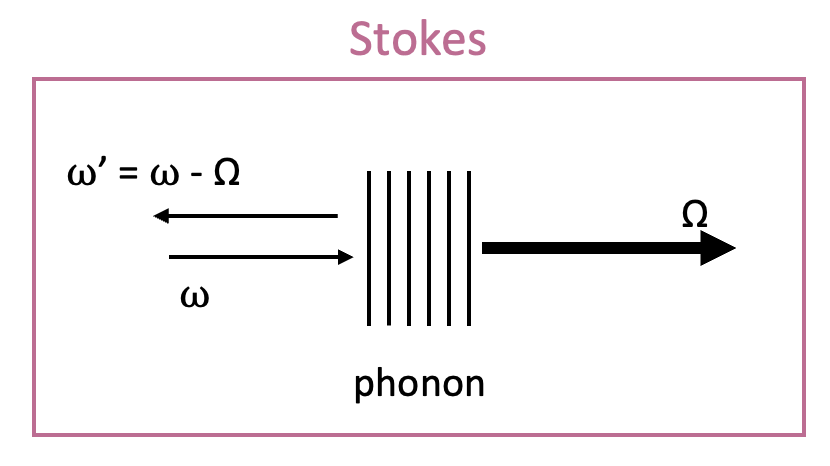
\includegraphics[width=\textwidth]{figs/3-Cooling/StokesHeatingProcess.png}
        \caption{}
        \label{fig:Cooling:StokesHeating}
    \end{subfigure}
    \hfill
    \begin{subfigure}[b]{0.49\textwidth}
        \centering
        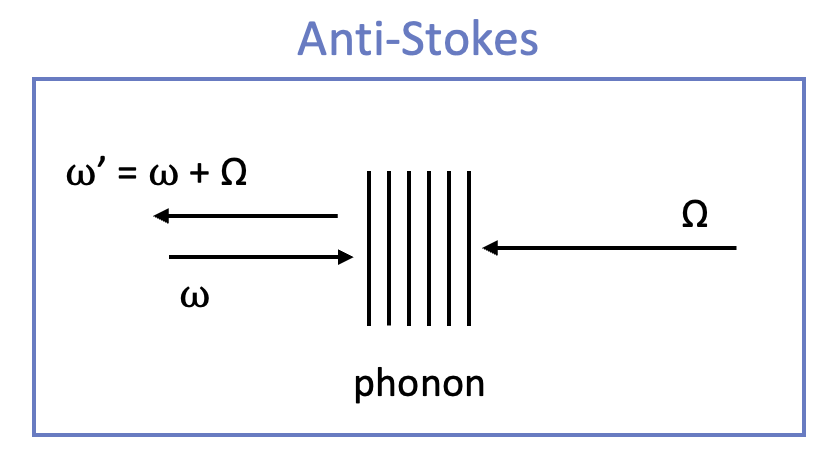
\includegraphics[width=\textwidth]{figs/3-Cooling/anti-StokesCoolingProcess.png}
        \caption{}
        \label{fig:Cooling:anti-StokesCooling}
    \end{subfigure}
    \caption{Illustration of optomechanical heating and cooling processes. Figure \ref{fig:Cooling:StokesHeating} shows an incident photon of frequency \(\omega\) scattering with a retreating phonon of frequency \(\Omega\), resulting in the annihilation of the incident photon and the creation of both an additional retreating phonon of frequency \(\Omega\) and a backwards propagating photon of reduced frequency and thereby energy (\(\omega_{\mathrm{Stokes}} = \omega - \Omega\)). Figure \ref{fig:Cooling:anti-StokesCooling} shows the inverse process, whereby an incident photon, \(\omega\), scatters with an approaching phonon, \(\Omega\), annihilating the incident photon and the phonon to produce a backwards propagating photon of increased frequency and thereby energy (\(\omega_{\mathrm{anti-Stokes}} = \omega + \Omega\)).}
    \label{fig:Cooling:StokesProcesses}
\end{figure}

The anti-Stokes process is the inverse process, whereby an \textit{approaching} phonon of frequency \(\Omega\) scatters with an incident photon of frequency \(\omega\), annihilating the \textit{phonon} and creating a backscattered photon at the addition energy (\(\omega_{\mathrm{anti-Stokes}} = \omega + \Omega\)). Both energy and momentum are again conserved, however in the anti-Stokes process, the incident light experiences a doppler \textit{up}-shift in frequency as if, to continue the analogy, the photon were reflected from an approaching mirror.

\subsection{Spectral Signatures of Cooling and Heating}
\label{Cooling:subsec:SpectralSignaturesofCoolingandHeating}
%v
Optomechanical cooling reduces the phonon occupation of a given mechanical mode. Evidence of this phenomenon is offered by changes in two key spectral features of the backscattered light: linewidth and amplitude. Spectral linewidth is a measure of the mechanical dissipation rate of the phonon mode. A broader linewidth corresponds with a higher mechanical dissipation rate of a given mode. Thereby, a reduction in phonon occupancy causes broadening of spectral linewidth while an increase in phonon occupancy causes linewidth narrowing. Spectral amplitude provides additional evidence of optomechanical cooling. Spectral amplitude is a measure of the scattered power produced from scattering of pump light with phonons occupying a given mechanical mode. Higher phonon occupancy within a given mode provides a higher rate of scattering and thus a higher measured spectral amplitude of the backscattered light. Increasing pump power reduces the phonon population occupying the anti-Stokes mode and thereby lessens the otherwise scattered power, measured as spectral amplitude. The inverse process occurs for the Stokes process; increasing pump power increases the phonon population occupying the Stokes mode and thereby increases the otherwise scattered power, measured by spectral amplitude.

In the spontaneous Brillouin scattering process, however, scattered power increases not only with phonon population (linked to temperature), but also with pump power \(P_{\mathrm{P}}\) (see Equation~\ref{eq:sponBSscatteredPower} in Appendix~\ref{appendix:comparison}). As a result, both the Stokes and anti-Stokes spectral amplitudes increase with increasing pump power. However, evidence of laser cooling is still given by spectral amplitudes in the form of assymetric growth rates of the Stokes and anti-Stokes spectra with increasing pump power. The anti-Stokes scattering process leads to a sublinear growth trend in peak spectral amplitudes with increasing pump power, whereas the Stokes process leads to superlinear growth.
%^
\section{Methods}
\label{Cooling:sec:Methods}

While spontaneous Brillouin scattering processes naturally alter phonon populations (and thus mode temperatures), practical demonstration and detection of these effects pose significant challenges. Foremost among these is the requirement to remain in the spontaneous regime: we wish to probe the natural thermal phonons in a medium, so we cannot rely on artificially driving the mechanical modes to enhance scattered power (see Appendix~\ref{appendix:comparison}, and specifically Figure~\ref{fig:SponBSvsStimBSvsCoBS}, for a comparison of scattered power produced by different Brillouin techniques). Although stimulated Brillouin scattering (SBS) is often employed to boost signal levels, it actively drives phonon populations via injected optical fields, and thus no longer measures the intrinsic thermal phonons. In practical terms, SBS occurs when the overall process gain factor \(G = G_{\mathrm{B}}P_{\mathrm{P}}L\) (where \(G_{\mathrm{B}}\) is the effective Brillouin gain, \(P_{\mathrm{P}}\) the pump power, and \(L\) the effective length) far exceeds unity (\(G \gg 1\)).

To demonstrate optomechanical cooling (i.e., an anti-Stokes process that lowers phonon energy), one must detect scattered light from a mode whose phonon population has been reduced. This is intrinsically difficult because a decreased phonon population means fewer scattering events, and hence diminished backscattered light. Consequently, an ideal testbed should provide sufficiently high single-pass gain (overall gain factor near unity) to enable clear detection, yet remain below the threshold that would drive the process into the stimulated regime. Achieving this balance ensures that measurements reflect genuine spontaneous cooling of a thermally populated phonon mode, rather than an artifact of optically driven phonons.

In addition to the requirement that the overall process gain be near but below unity, temporal constraints impose further critical conditions. Specifically, the rate at which phonons are removed from the system must exceed the rate at which they are replenished by the thermal bath to ensure net cooling of the anti-Stokes mode. This condition demands that backscattered photons leave the system rapidly, carrying away the extracted mechanical energy. A mean-field analysis (see Appendix~A of Johnson et al. (2023) \cite{johnson2023laser}) shows that the relevant depletion rate is \(4v_{\mathrm{g}}/L\), where \(v_{\mathrm{g}}\) is the group velocity of the anti-Stokes light and \(L\) is the system length. This must exceed the mechanical dissipation rate \(\Gamma_{\mathrm{0}}\), which represents the natural return of the phonon mode to thermal equilibrium. Hence, a suitable platform for demonstrating optomechanical cooling of traveling-wave phonons must fulfill the fast escape condition \(4v_{\mathrm{g}}/L > \Gamma_{\mathrm{0}}\). Meeting this requirement on system length, however, directly conflicts with the desire for a sufficiently high overall gain factor, illustrating the delicate balance needed for effective cooling.

%--------------------------------------------------------------------%

\subsection{\texorpdfstring{$CS_{2}$}{CS2}-Filled Liquid-Core Optical Fiber}
\label{Cooling:subsec:CS2FilledLCOF}

\begin{figure}[t]
  \centering
  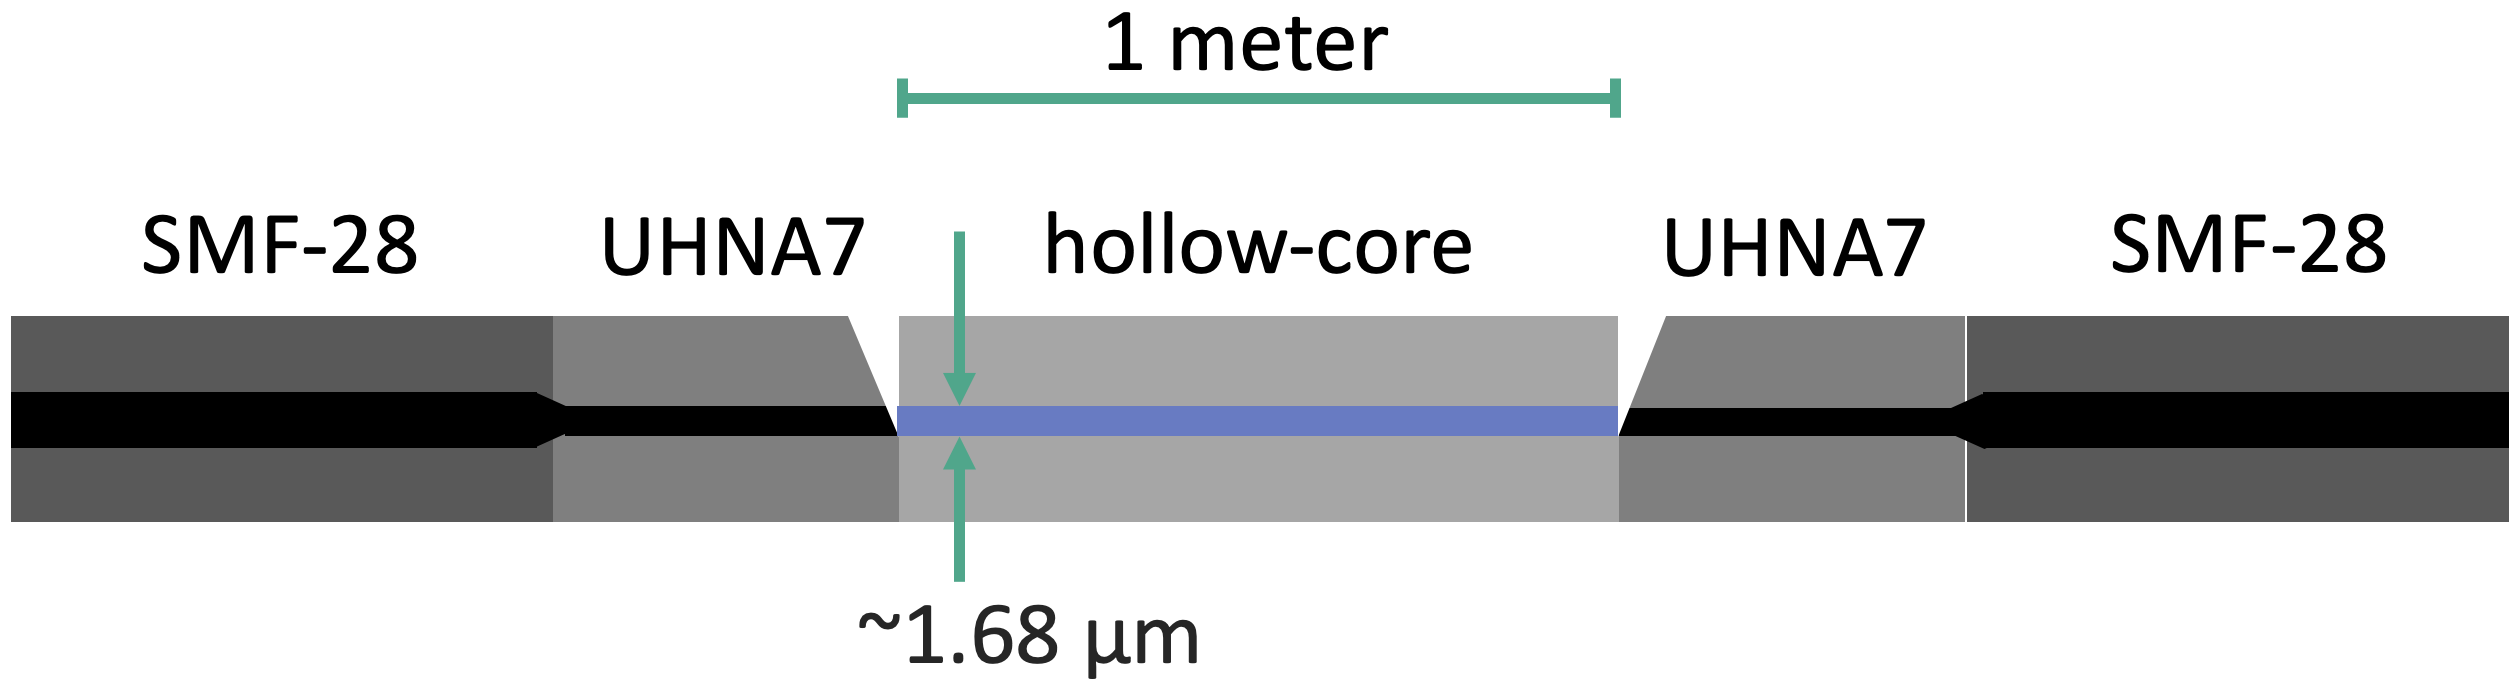
\includegraphics[width=\textwidth]{figs/3-Cooling/LCOFdiagram.png}
  \caption{Schematic of \ac{LCOF} design. A length of \ac{SMF-28} is arc-spliced to 5-\SI{10}{\centi\meter} of \ac{UHNA7} fiber, with a post-arc process applied to taper the larger \ac{SMF-28} core down to the smaller \ac{UHNA7} core for better mode matching and coupling efficiency. The \ac{UHNA7} fiber is angle-cleaved and fusion-spliced to a flat-cleaved hollow-core fiber via a heated filament in a Vytran fusion splicer system. The angle cleave results in a splice that only partially fuses the two fibers, leaving a pathway for liquid to enter the hollow core fiber via capillary action once submerged. A mirrored splice configuration on the other end of the length of hollow-core fiber allows air to escape as the fiber fills, and a reverse taper again provides improved mode matching for the light to recouple into \ac{SMF-28}.}
  \label{fig:LCOF diagram}
\end{figure}

To demonstrate optomechanical cooling of traveling wave phonons, we utilize \SI{1}{\meter} of \acl{LCOF} filled with carbon disulfide, first developed by Kieu et al. (2012). \cite{kieu2012integrated} This platform features large optomechanical coupling due to the high electrostritive response of \ce{CS2} \cite{boyd2020nonlinear} and the small effective area defining acousto-optic mode overlap offered by the small \SI{0.9}{\micro\meter} core radius of the capillary fiber. These characteristics of the \ac{LCOF} system combine to produce an effective Brillouin gain coefficient \(G_{\mathrm{B}} \sim\)\SI{2.3}{\per\watt\per\meter}, enabling sufficient scattering within the relatively short length required to satisfy the fast-escape condition \(4v_{\mathrm{g}}/L > \Gamma_{\mathrm{0}}\) (\(4v_{\mathrm{g}}/L \approx\) \SI{0.82}{\giga\hertz} and \(\Gamma_{\mathrm{0}} \approx\) \SI{0.61}{\giga\hertz}). \cite{johnson2023laser} Additionally, this \ce{CS2}-filled \ac{LCOF} system provides excellent acoustic and optical guidance due to the large electromagnetic and acoustic impedance differential between the \ce{CS2} core and surrounding silica. \cite{behunin2019spontaneous}

Figure~\ref{fig:LCOF diagram} shows a schematic of the \ac{LCOF} design. Coupling into and out of the \ac{LCOF} is facilitated by a short length of tapered \ac{UHNA7} for better mode matching between the \SI{4.8}{\micro\meter} core radius \ac{SMF-28} and the \SI{0.84}{\micro\meter} core radius of the capillary fiber. An angled cleave of the \ac{UHNA7} fiber allows for a small wedge gap to remain after fusion splicing to the capillary fiber. This gap allows liquid \ce{CS2} to enter and fill the hollow core of the capillary fiber via capillary action. Appendix~\ref{Cooling:Appendix:sec:FabricationofCS2FilledLCOF} describes the fabrication and filling processes of the \ac{LCOF} and details key insights which contributed to significant reductions in failure rate as well as time and material cost of sample preparation.

%--------------------------------------------------------------------%

\subsection{Experiment A: Spontaneous Brillouin Cooling}
\label{Cooling:subsec:ExperimentASpontaneousBrillouinCooling}

We conducted two independent experiments to demonstrate and verify laser cooling of traveling wave phonons in our \ce{CS2}-\ac{LCOF} platform. The first experiment (Experiment~A) employs a pump laser to launch \SI{1.55}{\micro\meter} light into the \ac{LCOF}. The backscattered Stokes and anti-Stokes components are filtered and collected by a detector. In this experiment, evidence of cooling is given by symmetry breaking between the amplitudes and widths of the Stokes and anti-Stokes spectra as pump power is varied.

Figure~\ref{fig:Cooling:ExperimentADesign} shows a schematic diagram of the experimental setup for Experiment~A. A \ac{CW} pump laser emitting at \SI{1.55}{\micro\meter} (\(\omega_{P}\)) is amplified by an \ac{EDFA} and its power is controlled by a \ac{VOA}. This light is subsequently routed via a circulator to the \ce{CS2}-\ac{LCOF}, where some of the light backscatters within the length of the \ac{LCOF}. Backscattered light is frequency-shifted, up for anti-Stokes (\(\omega_{\mathrm{aS}} = \omega_{\mathrm{P}} + \Omega_{\mathrm{B}}\)) and down for Stokes
(\(\omega_{\mathrm{S}} = \omega_{\mathrm{P}} - \Omega_{\mathrm{B}}\)),
by a band of frequencies centered around the Brillouin frequency of the \ac{LCOF} (\(\Omega_{\mathrm{B,\,LCOF}} \approx\) \SI{2.27}{\giga\hertz}). Backscattered light is routed by circulators to a \SI{5}{\giga\hertz} \ac{BPF} to allow selection of either the Stokes or anti-Stokes light while also reducing unwanted frequency noise. The filtered signal is then incident on a photodiode detector sensitive to \si{\giga\hertz} frequencies. A \ac{LO} is synthesized from the pump laser, polarization controlled, amplified, and combined with the signal pre-detector for heterodyne detection. Output from the detector is amplified with a \ac{RF} amplifier and sent to a \ac{RFSA} for data collection.

To conduct the experiment, pump power was varied from \SI{10}{\milli\watt} to \SI{290}{\milli\watt} in increments of \SI{10}{\milli\watt}, as measured pre-injection into the \ac{LCOF}, and respective Stokes and anti-Stokes spectra for each pump power were collected sequentially by tuning the placement of the \ac{BPF}. Optical transmission through the entire \ac{LCOF} sample which was used for the published data was measured to be 17\%, giving \(100\sqrt{0.17} \approx 41\%\) transmission through just the first splice assuming equal transmission through both \ac{LCOF} splices. This provides a scaling factor for obtaining intrafiber powers from injected pump power (\(P_{\mathrm{intrafiber}} = \sqrt{0.17}P_{\mathrm{P}}\)) which was used for data processing and analysis.

\begin{figure}[t]
  \centering
  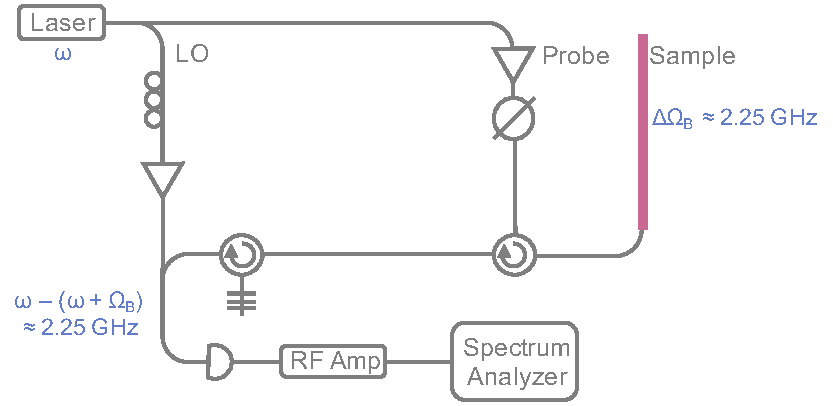
\includegraphics[width=\textwidth]{figs/3-Cooling/pumpOnlyDesign.pdf}
  \caption{Schematic of experimental setup for Experiment~A. In this experiment, a \ac{CW} pump laser emitting at \SI{1.55}{\micro\meter} is amplified, passed through a circulator, and injected into the \ce{CS2}-\ac{LCOF}. Backscattered light is routed to a \ac{BPF} for selection of Stokes or anti-Stokes frequencies and sent to a detector. A \ac{LO} is synthesized from the pump laser for heterodyne detection, whereby a \acl{PC} is used to align the polarization of the \ac{LO} to that of the backscattered signal. The signal passes through a \acl{RF} amplifier before being sent to a \ac{RFSA} for collection. Pump power is controlled by a \ac{VOA} placed just after the \ac{EDFA}. Stokes and anti-Stokes spectra are collected sequentially for each pump power by adjusting the placement of the \ac{BPF}.}
  \label{fig:Cooling:ExperimentADesign}
\end{figure}

\subsection{Experiment B: Pump-Probe Verification}
\label{Cooling:subsec:ExperimentBPump-ProbeVerification}

A second experiment (Experiment~B) was conducted to provide direct evidence of cooling via a pump-probe spectroscopy technique, whereby a separate probe laser is held at constant power while a pump laser is varied to affect cooling in the \ac{LCOF}. In Experiment~B, backscattered light from the probe laser provides direct evidence of cooling through spectral changes in amplitude and width as pump power is independently varied. To achieve independence of the pump and probe, probe light was controlled to be polarized orthogonal to the pump.

Figure~\ref{fig:Cooling:ExperimentBDesign} shows a schematic of the experimental design for Experiment~B. Starting from a single \ac{CW} laser operating at \SI{1.55}{\micro\meter}, we generate a pump \(\omega_{\mathrm{P}}\), probe \(\omega_{\mathrm{Pr}}\), and \ac{LO}. A \ac{PBS} combines the pump and probe for co-injection into the \ac{LCOF}. The pump light is amplified by an \ac{EDFA}, and its polarization is adjusted so that it reflects at the \ac{PBS} for launching into the \ac{LCOF}. The probe light passes through a circulator and is polarization-adjusted to transmit through the \ac{PBS} for injection into the \ac{LCOF}. A 99-1 splitter directs 1\% of the combined pump and probe light to a second \ac{PBS} for monitoring of respective powers injected into the \ac{LCOF}.

\begin{figure}[t]
  \centering
  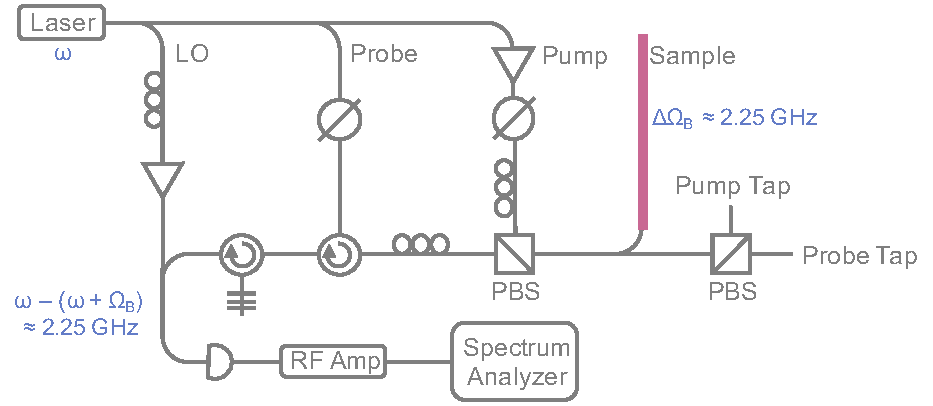
\includegraphics[width=\textwidth]{figs/3-Cooling/pumpProbeDesign.pdf}
  \caption{Schematic of experimental setup for Experiment~B. A pump, probe, and \ac{LO} are generated from a single \ac{CW} laser operating at \SI{1.55}{\micro\meter}. Pump light is amplified and directed through a \ac{VOA} and \ac{PC}, where its polarization is adjusted to reflect at the \ac{PBS}. Probe light passes through a \ac{VOA} for careful power control across measurement sets before being routed by a circulator to the \ac{PBS}. Polarization of the probe light is adjusted for transmission through the \ac{PBS} for co-injection with the pump into the \ac{LCOF}. A 99-1 splitter directs 1\% of the total pump and probe light to a second \ac{PBS} for monitoring of respective powers injected injected into the \ac{LCOF}. Backscattered Stokes and anti-Stokes components of both the pump and the probe retrace to the first \ac{PBS}, where the respective polarization states of each ensure a re-separation of backscattered pump and probe light. The probe light is filtered by a tunable \ac{BPF} and heterodyned with the \ac{LO} prior to detection. Detector output is amplified by an \ac{RF} amplifier and fed to an \ac{RFSA} for data collection.}
  \label{fig:Cooling:ExperimentBDesign}
\end{figure}

Backscattered light from both pump and probe is shifted in frequency by approximately the Brillouin frequency of the \ac{LCOF} (\(\Omega_{\mathrm{B,\,LCOF}} \approx \SI{2.27}{\giga\hertz}\)). The Stokes components (downshifted) satisfy

\begin{equation}
\omega_{\mathrm{P,\,S}} = \omega_{\mathrm{P}} - \Omega_{\mathrm{B}},
\quad
\omega_{\mathrm{Pr,\,S}} = \omega_{\mathrm{Pr}} - \Omega_{\mathrm{B}},
\end{equation}
\\
while the anti-Stokes components (upshifted) satisfy

\begin{equation}
\omega_{\mathrm{P,\,aS}} = \omega_{\mathrm{P}} + \Omega_{\mathrm{B}},
\quad
\omega_{\mathrm{Pr,\,aS}} = \omega_{\mathrm{Pr}} + \Omega_{\mathrm{B}}.
\end{equation}
\\
These four backscattered signals are centered within a band of frequencies due to the finite phonon lifetime in the \ac{LCOF}. The polarization state of the backscattered pump and probe light is recovered after retracing their paths, permitting only probe light to transmit through the \ac{PBS} for filtration and heterodyne detection. Output from the detector is again amplified by an \ac{RF} amplifier and routed to an \ac{RFSA} for data collection. With the probe power inside the \ac{LCOF} held constant, changes in the amplitude and width of the probe spectra provide direct evidence of laser cooling from varying pump powers within the \ac{LCOF}.

%--------------------------------------------------------------------%

\section{Results}
\label{Cooling:sec:Results}


\subsection{Experiment A Results}
\label{Cooling:subsec:ExperimentAResults}

Figures~\ref{fig:Cooling:P-O Stokes} and \ref{fig:Cooling:P-O anti-Stokes} show the respective Stokes and anti-Stokes spectra gathered across a range of intra-fiber pump power from \SI{4.12}{\milli\watt} to \SI{119.57}{\milli\watt}. Both Stokes and anti-Stokes spectra sets are centered at approximately \(f_{B} = \) \SI{2.27}{\giga\hertz}, representing a respective up- and downshift from the pump frequency by the Brillouin frequency of the \ce{CS2}-\ac{LCOF} at \SI{1.55}{\micro\meter}. For increasing pump power, we see an asymmetry in evolution of peak spectral densities and linewidths of the Stokes and anti-Stokes spectra, key fingerprints of optomechanical cooling. The peak amplitudes of the anti-Stokes spectra increase sublinearly while that of the Stokes increase superlinearly (Figure~\ref{fig:Cooling:P-O Heights vs Pow}). As phonon occupation decreases (cooling) in the anti-Stokes phonon mode, the rate of scattering also decreases due to the diminished population of phonons able to participate in scattering. A lesser rate of scattering produces less backscattered light incident on the detector, causing the peak spectral density to be less than if no cooling had occured. The opposite effect occurs in the Stokes process; as phonon occupation increases (heating) in the Stokes phonon mode, the rate of scattering also increases owing to a bolstered number of phonons available to participate in scattering. This increased rate of scattering results in more backscattered light collected by the detector and causing the peak spectral density to be greater than if no heating had occured. Critically, since scattered power is also dependent on pump power (see Equation~\ref{eq:sponBSscatteredPower}), the peak amplitude of both processes increases with increasing pump power. However, the sublinear (superlinear) growth rate in peak amplitude of the anti-Stokes (Stokes) spectra as pump power increases provides key evidence of optomechanical cooling (heating) of the respective \ac{LCOF} phonon modes.

\begin{figure}[t]
  \centering
  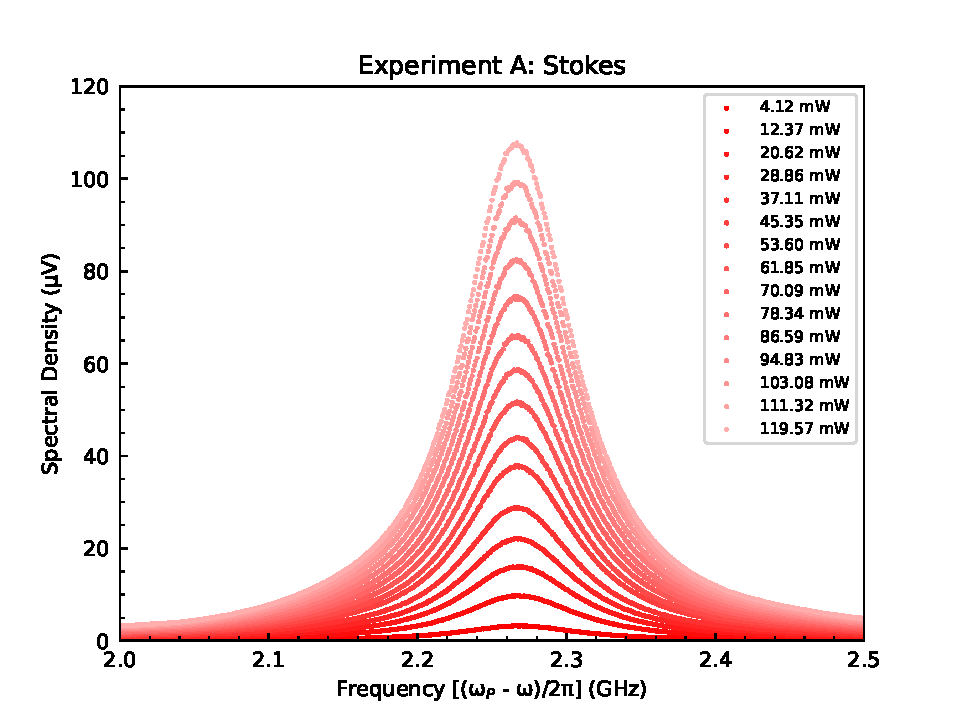
\includegraphics[width=\textwidth]{figs/3-Cooling/P-O Stokes.pdf}
  \caption{.}
  \label{fig:Cooling:P-O Stokes}
\end{figure}

%Table Stokes

\begin{figure}[t]
  \centering
  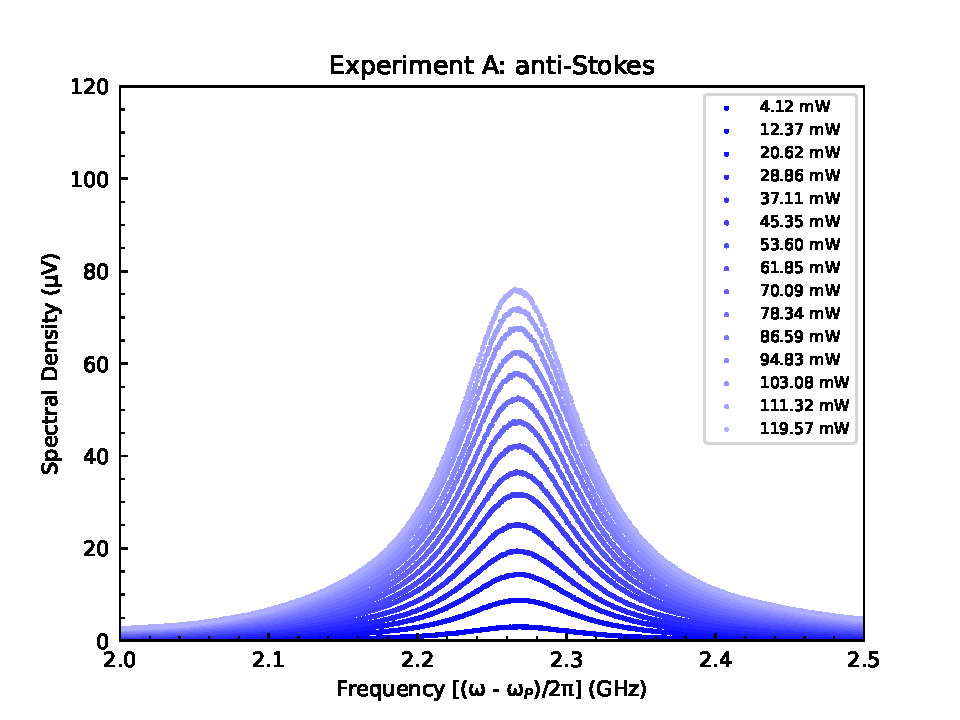
\includegraphics[width=\textwidth]{figs/3-Cooling/P-O anti-Stokes.pdf}
  \caption{.}
  \label{fig:Cooling:P-O anti-Stokes}
\end{figure}

%Table anti-Stokes

\begin{figure}[t]
  \centering
  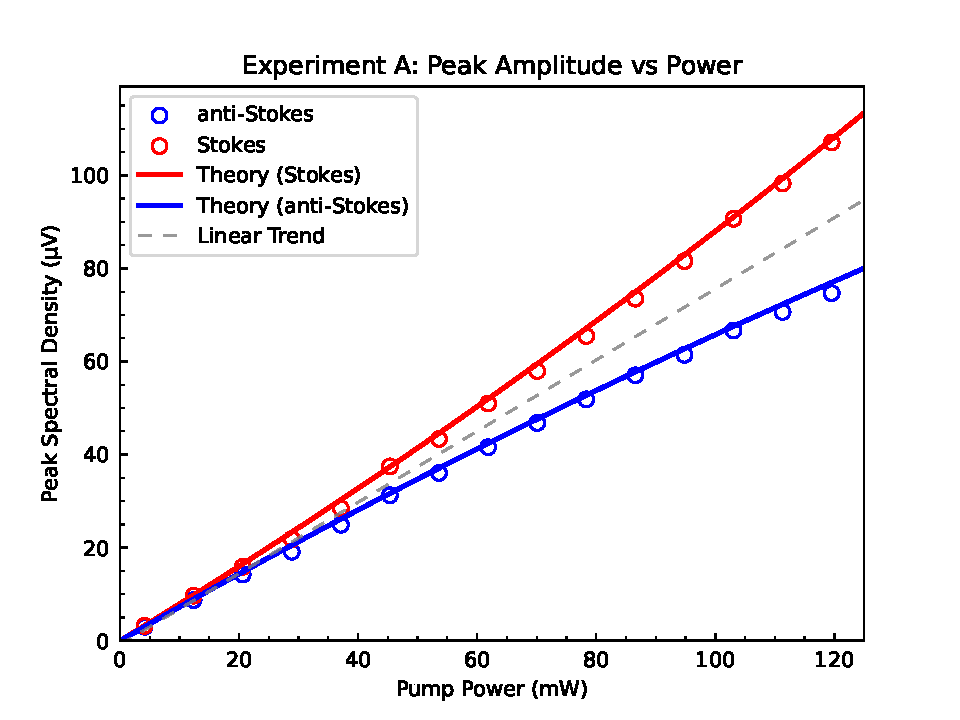
\includegraphics[width=\textwidth]{figs/3-Cooling/P-O Heights vs Pow.pdf}
  \caption{.}
  \label{fig:Cooling:P-O Heights vs Pow}
\end{figure}

\begin{figure}[t]
  \centering
  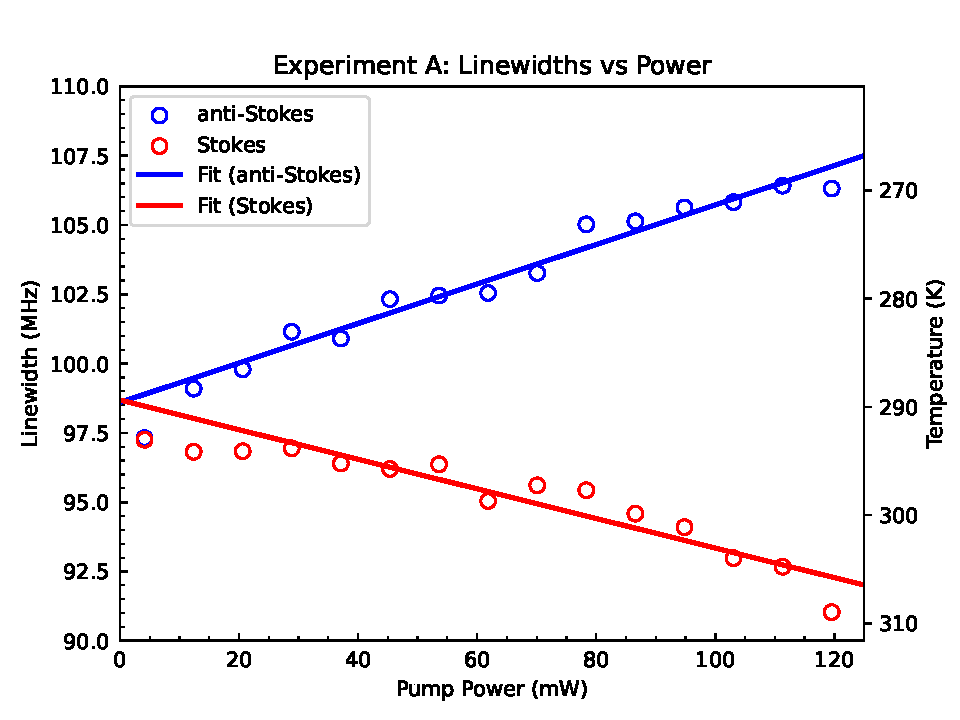
\includegraphics[width=\textwidth]{figs/3-Cooling/P-O Linewidths.pdf}
  \caption{.}
  \label{fig:Cooling:P-O Linewidths}
\end{figure}

\begin{figure}[t]
  \centering
  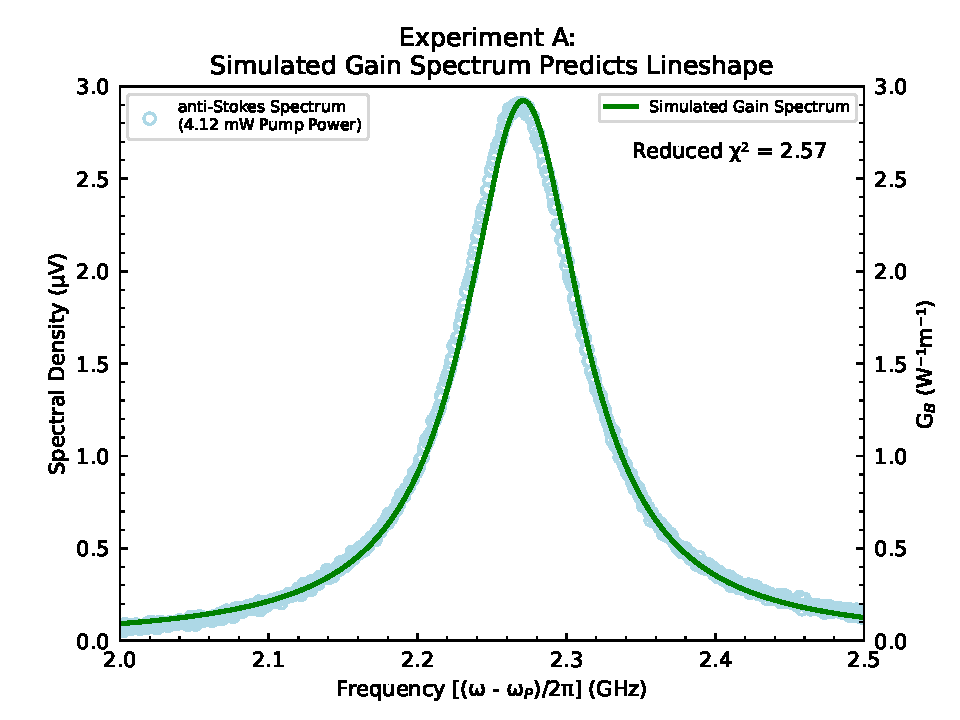
\includegraphics[width=\textwidth]{figs/3-Cooling/P-O Simulated Gain.pdf}
  \caption{.}
  \label{fig:Cooling:P-O Simulated Gain}
\end{figure}


\subsection{Experiment B Results}
\label{Cooling:subsec:ExperimentBResults}

\begin{figure}[t]
  \centering
  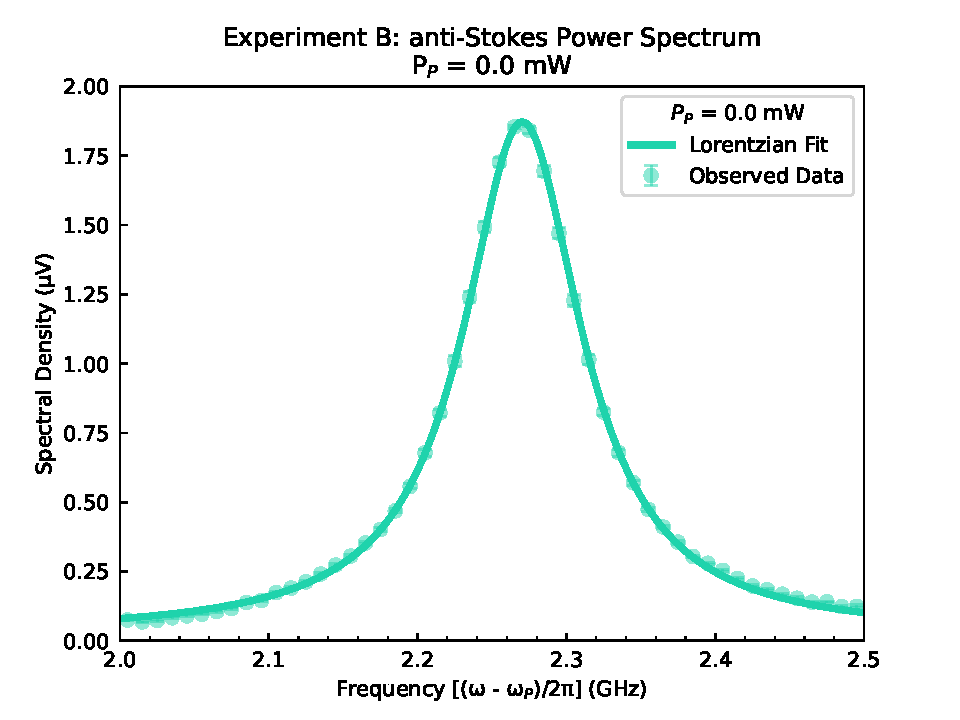
\includegraphics[width=\textwidth]{figs/3-Cooling/P-P anti-Stokes Fit - 0mW.pdf}
  \caption{.}
  \label{fig:Cooling:P-P anti-Stokes Fit - 0mW}
\end{figure}

\begin{figure}[t]
  \centering
  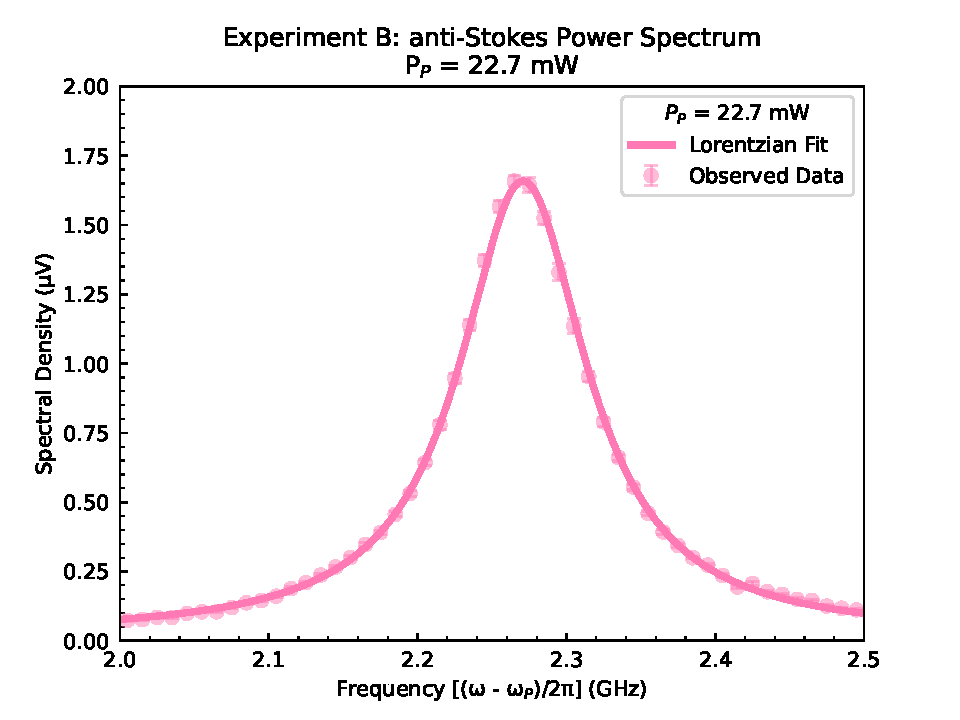
\includegraphics[width=\textwidth]{figs/3-Cooling/P-P anti-Stokes Fit - 55mW.pdf}
  \caption{.}
  \label{fig:Cooling:P-P anti-Stokes Fit - 55mW}
\end{figure}

\begin{figure}[t]
  \centering
  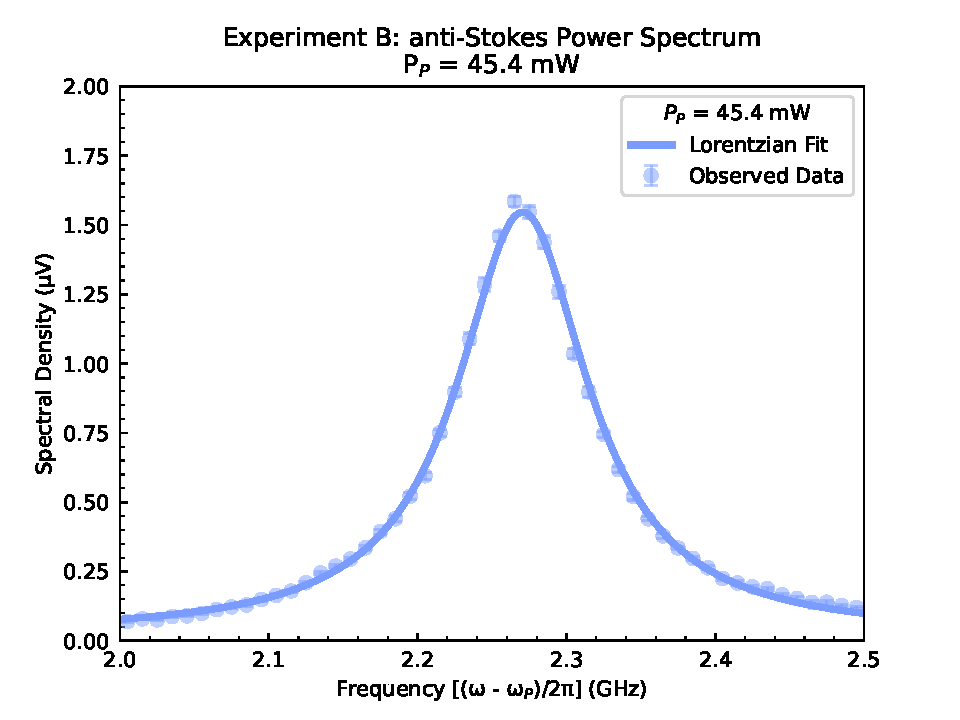
\includegraphics[width=\textwidth]{figs/3-Cooling/P-P anti-Stokes Fit - 110mW.pdf}
  \caption{.}
  \label{fig:Cooling:P-P anti-Stokes Fit - 110mW}
\end{figure}

\begin{figure}[t]
  \centering
  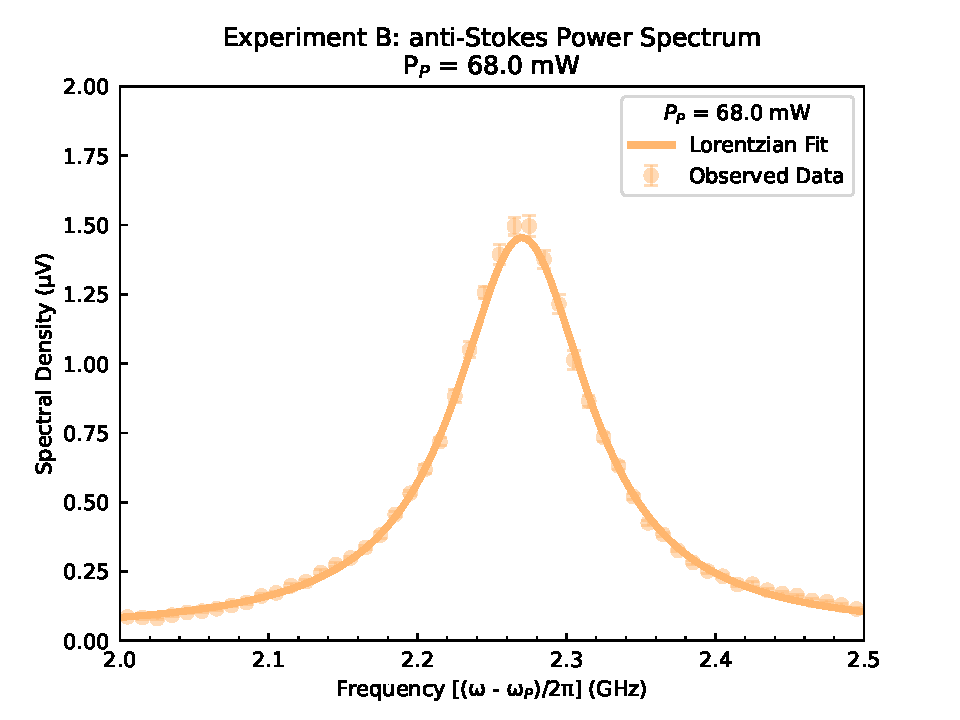
\includegraphics[width=\textwidth]{figs/3-Cooling/P-P anti-Stokes Fit - 165mW.pdf}
  \caption{.}
  \label{fig:Cooling:P-P anti-Stokes Fit - 165mW}
\end{figure}

\begin{figure}[t]
  \centering
  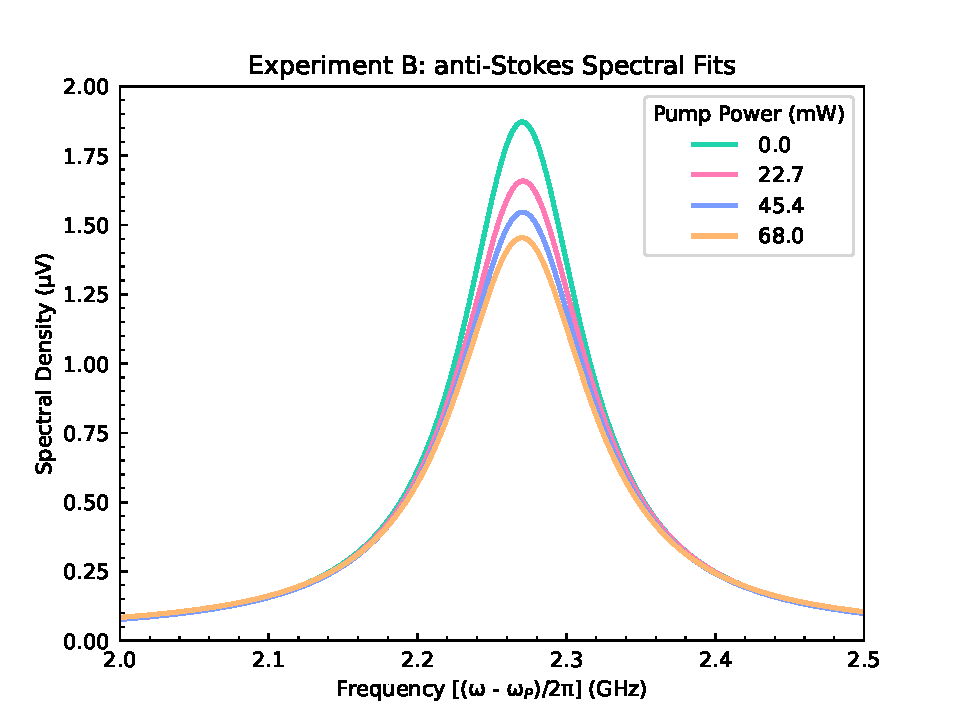
\includegraphics[width=\textwidth]{figs/3-Cooling/P-P anti-Stokes Fits.pdf}
  \caption{.}
  \label{fig:Cooling:P-P anti-Stokes Fits}
\end{figure}

\begin{figure}[t]
  \centering
  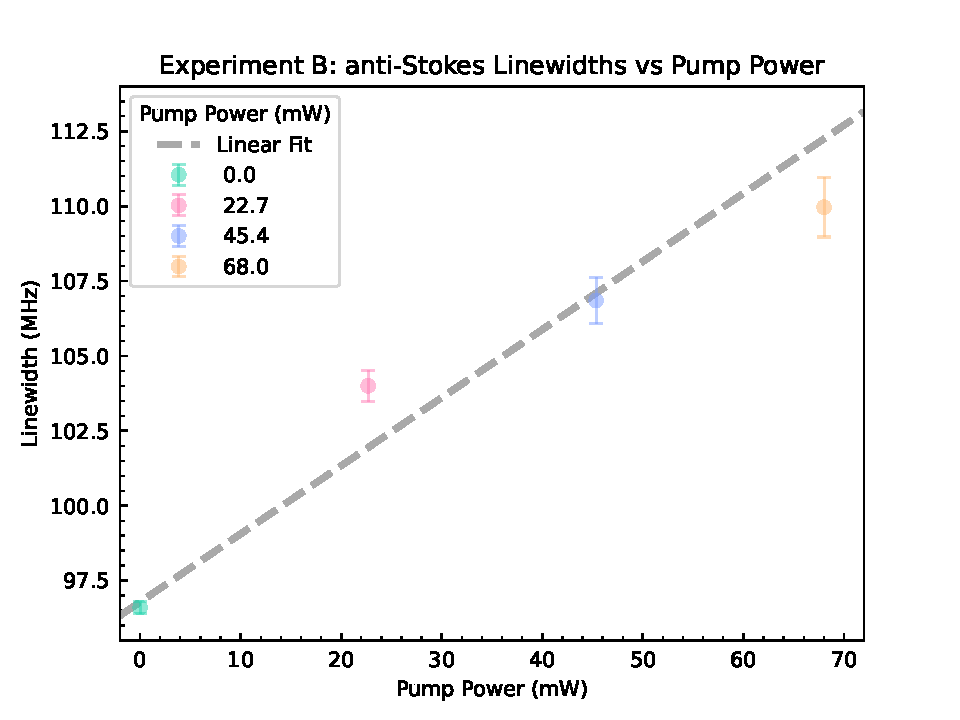
\includegraphics[width=\textwidth]{figs/3-Cooling/P-P anti-Stokes Wid v Pow.pdf}
  \caption{.}
  \label{fig:Cooling:P-P anti-Stokes Wid v Pow}
\end{figure}

\begin{figure}[t]
  \centering
  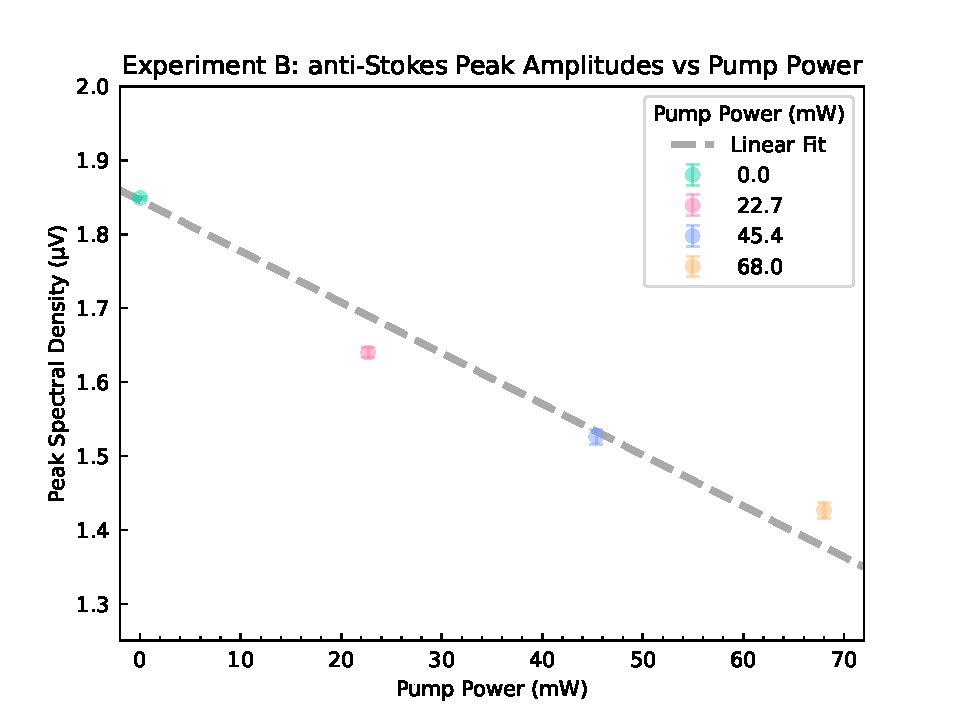
\includegraphics[width=\textwidth]{figs/3-Cooling/P-P anti-Stokes Height v Pow.pdf}
  \caption{.}
  \label{fig:Cooling:P-P anti-Stokes Height v Pow}
\end{figure}

\subsection{Evidence of Transmission Degradation}
\label{Cooling:subsec:Evidence of Transmission Degradation}

After comparing the anti‐Stokes linewidths measured in Experiments~A and B, we conclude that significant splice transmission degradation occurred in the interim. Experiment~B was performed first (with a through‐fiber transmission of 17\%), followed by Experiment~A the next day. If the experimental conditions were unchanged between the two experiments, the slopes of the anti‐Stokes linewidth versus pump power would be identical (Figures~\ref{fig:Cooling:P-O Linewidths} and \ref{fig:Cooling:P-P anti-Stokes Wid v Pow}). Instead, Experiment~B exhibits a noticeably steeper slope than Experiment~A. A reanalysis shows that reducing the assumed transmission for Experiment~A so the two slopes match would require the total fiber transmission to have dropped from 17\% down to approximately 3\%. While large, this degradation is plausible and is supported by several further observations.

First, the fiber immediately following the exit splice of the \ac{LCOF} broke off after initially measuring the transmission and before performing Experiment~B, making it no longer possible to remeasure the full through‐fiber transmission during Experiment~A. If that transmission had declined in the meantime, we had no direct means to detect it. Additionally, during both experiments, the pump power was recorded via a 1\% tap prior to launching into the \ac{LCOF}. Hence, any losses incurred at the damaged splice were not accounted for. As a result, if the splice transmission had indeed worstened, we overestimated the actual intracore power in Experiment~A.

Further quantitative analysis supports this hypothesis as well. As we reported in Johnson et al. (2023)\cite{johnson2023laser}, Experiment~A yields a Brillouin gain of approximately \SI{2.3}{\per\watt\per\meter}, calculated using\cite{johnson2023laser}

\begin{equation}
  \Gamma \approx \Gamma_{0}\left(1 - \frac{1}{4}G\right),
\end{equation}

where \(\Gamma\) is the optically-altered phonon dissipation rate, \(\Gamma_{0}\) is the equilibrium phonon dissipation rate, and \(G\) is the overall process gain factor \(G = G_{B}P_{P}L\) (see Section~\ref{appendix:comparison}). This value is smaller than the \SI{6(1)}{\per\watt\per\meter} reported by Behunin et al. in 2019\cite{behunin2019spontaneous} for a near‐identical \ac{LCOF} geometry and fabrication method. If instead we calculate the Brillouin gain based on the linewidths and corresponding intrafiber pump powers seen in Experiment~B, we find the Brillouin gain to be approximately \SI{8(2)}{\per\watt\per\meter}, which is in excellent agreement with the prior published value from the literature. In estimating the uncertainty here, we have taken the \(2\sigma\) confidence level in linewidths and allowed a 10\% uncertainty in intracore pump powers. The natural conclusion is that for Experiment~A we overstated the intrafiber pump power due to previously unknown and significant splice transmission degradation between experiments. This produced an apparent smaller dependence of linewidth on pump power in Experiment~A, thereby producing an under-reporting of the true gain of the \ac{LCOF} in the published paper.

Finally, the linewidth vs power plots appear to exhibit a slight sublinear trend (especially that of Experiment B), but any saturation effect or similar which could cause a sublinear trend in linewidths with pump power should activate at the same intracore optical power. However, with our two data sets, a slight sublinear trend invoked by the much higher pump powers used in Experiment~A should then not cause the same saturation effect for the much lower pump powers used in Experiment~B, if the optical transmission were the same across experiments. If instead the transmission of the \ac{LCOF} splice at entrance had been significantly greater for the earlier-run Experiment~B than for Experiment~A, the intracore powers for Experiment~B could have been similar or far greater than the those for Experiment~A. This might explain why Experiment~B linewidths appear to exhibit slightly sublinear growth with pump power despite the lower pump powers launched into the \ac{LCOF}. Experiment~A in fact does not seem to exhibit as apparent of a sublinear growth trend in linewidths as is seen for Experiment~B. This is consistent with an approximate factor of 5 drop in transmission through the \ac{LCOF} splice at the time Experiment~A was performed, as indicated by the discrepancy in linewidth growth rates between experiments.

In summary, all these lines of evidence indicate that the \ac{LCOF} splice transmission fell substantially between Experiments~B and A, on the order of a factor of five. This fully reconciles the differing slopes in the anti‐Stokes linewidth data and explains the otherwise surprising discrepancy in inferred Brillouin gain compared to values published in the literature for identical \ce{CS2}-filled \ac{LCOF}s.

%--------------------------------------------------------------------%

\section{Discussion}
\label{Cooling:sec:Discussion}

\subsection{Standardized Cooling Metric}
\label{Cooling:subsec:StandardizedCoolingMetric}

% need for normalized cooling metric - per pump power, and such that one cannot start a system in a heated state to achieve a greater stated cooling ability. Or maybe room temperature is identical across systems? check. if not, normalize.

\subsection{Alternative Platforms}
\label{Cooling:subsec:AlternativePlatforms}

Tapered chalcogenide Photonic Crystal Fiber: Max Plank Results (corroborate our results)

\subsection{Pathways to Net Cooling}
\label{Cooling:subsec:PathwaystoNetCooling}

Ideas to achieve net cooling, one might design a system where:

1) single pass gain bias
     swing energy transfer bias to favor anti-Stokes over Stokes (mode-dependent gain)
     the Stokes process were not permitted (ryan's only idea), or just significantly restricted - what is that bias threshold requirement?
     currently, we are net *heating* the system because it is easier to heat from equilibrium than cool (right? explore this. it's also hard to make it hotter beyond a certain point.)
     implementation ideas:
       multi-pump scheme to destructively interfere with Stokes and/or constructively interfere with anti-Stokes
       doping or specialized waveguide gratings that pick out the Stokes band for out-of-plane scattering

2) time bias
     create an energy transfer *rate* bias between Stokes and anti-Stokes
     can be accomplished with either the brillouin energy transfer rate or the repopulation rate

       brillouin process rate:
         4vg/L, have either group velocity or length be different for Stokes vs anti-Stokes (smaller vg or larger L for Stokes than anti-Stokes)
         make anti-Stokes fast light and/or Stokes slow light
         vg inversely proportional to pump power, so it's a balance
           increasing pump power = slower escape time (4vgL), and also larger dissipation (Gamma+)

       repopulation rate:
         thermally insulate the anti-Stokes mode from the thermal bath that would repopulate it
         or at least insulate it some amount more than Stokes (what is that threshold? even if it's only net cooled for picoseconds, what is that minimum crossover point insulation bias point)
         essentially locks in the cooled mode while letting the heated mode spill out
         implementation idea:
           design a fiber/waveguide with acoustic directional bias, such that phonons travelling one direction dissipate quicker because of the geometry/acoustic properties of the fiber. (triangles? acting as tapered acoustic dissipators, pointing in one direction?)

3) starting temperature
     Could you acieve net cooling in a cheap and dirty sense by starting the system in a very heated state, thus invoking a natural dissipation rate bias?! - yes!
     Things do naturally run hot, perhaps no extra fancy engineering is needed for some practical systems? (data processing, reduce thermal noise from above ambient heat)
     not traditional definition of optical refrigeration below ambient/thermal bath, but still *useful*
     is this already done? lit search

Think about a practical device or system for each of these cases (think waveguide playground!)

\subsection{Applications to Ground State Cooling}
\label{Cooling:subsec:ApplicationstoGroundStateCooling}
